%----------------------------------------------------------------
% Preamble
%----------------------------------------------------------------
\documentclass[12pt,aspectratio=169,xcolor=dvipsnames,hyperref={colorlinks=true,linkcolor=blue,citecolor=black}]{beamer}
%---------------------------------------------------------------
% Conditionals
%---------------------------------------------------------------
\usepackage{etoolbox}					 		% Toolbox of programming facilities
\usepackage{xpatch}						  		% Extends etoolbox patching commands

%---------------------------------------------------------------
% Paper
%---------------------------------------------------------------
\newtoggle{toclinks}				    	% When editing, add links (next to section titles) to ToC
\newtoggle{cboxes}					   		% When editing, write comments and to-dos
\newtoggle{fulldraft}					 	% Generate short (outline) and long (full draft) versions
\newtoggle{floatstxt}					 	% Put figures and tables in the text or at the end
\newtoggle{blind}					 		% Generate version for journal submission (no identifiers)
\newtoggle{revised}					 		% Highlight changes in revised version
\newtoggle{withappdx}					 	% Include appendix at the end of the paper

\settoggle{toclinks}{true}			   		% 'true' to include ToC and links
\settoggle{cboxes}{true}			   		% 'true' to include boxed comments
\settoggle{fulldraft}{true}	   	 	     	% 'false' to generate an outline
\settoggle{floatstxt}{true}	   	 	 		% 'true' to put figures and tables in the text
\settoggle{blind}{false}	   	 	 		% 'true' to generate version without identifiers
\settoggle{revised}{false}	   	 	 		% 'true' to highlight changes with color
\settoggle{withappdx}{true}	   	 	 		% 'true' to include appendix at the end. Caution: May need to compile paper.tex twice (for ToC) and re-run biber (for references) if the value of this toggle changes

%---------------------------------------------------------------
% Slides
%---------------------------------------------------------------
\newtoggle{stops}					   		% Generate version with stepwise uncovering (more slides)

\settoggle{stops}{true} 					% 'false' for version without stops

%---------------------------------------------------------------
% Paper vs Slides
%---------------------------------------------------------------
\newtoggle{longnotes}					   	% Standalone descrptions in floats: Long for paper, short for slides
\newtoggle{coloreq}					   		% Highlight parts of an equation in slides

\settoggle{longnotes}{true} 				% No need to change it: paper.tex uses it as 'true', each float file sets it to 'false'
\settoggle{coloreq}{false} 					% No need to change it: paper.tex uses it as 'false', slides.tex sets it to 'true' when needed		   		  					% Toggles
%% Packages for Beamer
% Fromatting, Math, Figures, Tables,
% Special Characters, Hyperlinks, References

%---------------------------------------------------------------
% Fromatting
%---------------------------------------------------------------
\usepackage[sfdefault,extralight]{FiraSans}		% To set Fira Sans as the default text font
	\renewcommand*\oldstylenums[1]{{\firaoldstyle #1}}
\usepackage{pgfpages}							% To display multiple pages on a single page (for notes)
\usepackage{setspace}							% Line spacing and spaces above/below equations
	\setstretch{1.7}
	\AtBeginDocument{							% Space before and after an equation
		\addtolength\abovedisplayskip{-0.5\baselineskip}
		\addtolength\belowdisplayskip{-0.5\baselineskip}}
\usepackage{appendixnumberbeamer}				% To restart the frame numbering in appendix
\usepackage{enumerate} 							% To customize the enumerate style
%\usepackage{enumitem} 							% To control list environments, but 'disturbs' beamer

%---------------------------------------------------------------
% Math
%---------------------------------------------------------------
\usepackage{amsmath} 					 		% For multi-line statements
\usepackage{amssymb} 					 		% For math symbols and fonts
\usepackage{dsfont}								% More math fonts (e.g. indicator function)
%\usepackage{amsthm}							% For theorems

%---------------------------------------------------------------
% Figures
%---------------------------------------------------------------
\usepackage{graphicx} 				 			% To include figures
\usepackage[outdir=./]{epstopdf} 	  			% To avoid errors when calling figures
\usepackage{subcaption}					  		% Multi-panel figure
\usepackage{tikz}								% To create high quality diagrams
%	\usetikzlibrary{arrows,calc,decorations,fit,matrix,positioning,shapes,tikzmark}

%---------------------------------------------------------------
% Tables
%---------------------------------------------------------------
\usepackage{tabularx}					 		% For paragraph-like columns
\usepackage{booktabs}			  	   			% For \toprule, \midrule, \bottomrule
\usepackage{multirow}			   				% To add entries with multiple rows
\usepackage{bigstrut} 			 	 		 	% To open up tabular spacing
\usepackage{siunitx}				 	  		% To align the decimal points
\usepackage{threeparttable}		 	  			% To include a structured note section

%---------------------------------------------------------------
% Special Characters
%---------------------------------------------------------------
\usepackage{pifont}								% Symbols
	\newcommand{\cmark}{\ding{51}}				% Checkmark
	\newcommand{\xmark}{\ding{55}}				% Xmark
\usepackage[utf8]{inputenc}			  		 	% Handles accented characters (same output on all systems)
\usepackage[T1]{fontenc}		  	  			% Fonts to use for printing characters
%\usepackage{underscore}				   		% Handles "_" in text but hurts filenames/labels with it

%---------------------------------------------------------------
% Hyperlinks
%---------------------------------------------------------------
\usepackage[absolute,overlay]{textpos}			% Positions text in slide (e.g. links to slides)
%\usepackage[colorlinks=true]{hyperref} 	 	% Loaded by default in Beamer; pass arguments in \documentclass

%---------------------------------------------------------------
% References
%---------------------------------------------------------------
%\usepackage[style=authoryear,backend=biber]{biblatex}	% Option 1
%\addbibresource{../References/library.bib} 			% Option 1
\usepackage[round,authoryear]{natbib}					% Option 2   		  					% Packages
%---------------------------------------------------------------
% Theme Colors
%---------------------------------------------------------------
\usepackage{xcolor}
	\definecolor{JHUblue}{rgb}{0.36, 0.54, 0.66}%{0, 0.45, 0.114}
	\definecolor{JHUgrey2}{rgb}{180, 178, 173}
	\definecolor{JHUorange}{rgb}{255, 105, 0}
	\definecolor{airforceblue}{rgb}{0.36, 0.54, 0.66}
	\definecolor{bluegray}{rgb}{0.4, 0.6, 0.8}
	\definecolor{cerulean}{rgb}{0.0, 0.48, 0.65}
	\definecolor{darkcerulean}{rgb}{0.03, 0.27, 0.49}
	\definecolor{darkpastelblue}{rgb}{0.47, 0.62, 0.8}
	\definecolor{glaucous}{rgb}{0.38, 0.51, 0.71}
	\definecolor{hanblue}{rgb}{0.27, 0.42, 0.81}
	\definecolor{iceberg}{rgb}{0.44, 0.65, 0.82}
	\definecolor{indigo}{rgb}{0.0, 0.25, 0.42}					% with infolines
	\definecolor{internationalkleinblue}{rgb}{0.0, 0.18, 0.65}
	\definecolor{lapislazuli}{rgb}{0.15, 0.38, 0.61}
	\definecolor{mediumelectricblue}{rgb}{0.01, 0.31, 0.59}		% Good
	\definecolor{mediumpersianblue}{rgb}{0.0, 0.4, 0.65}
	\definecolor{mediumtealblue}{rgb}{0.0, 0.33, 0.71}
	\definecolor{midnightblue}{rgb}{0.1, 0.1, 0.44}				% Cool dark
	\definecolor{navyblue}{rgb}{0.0, 0.0, 0.5}					% Darker than standard purple
	\definecolor{phthaloblue}{rgb}{0.0, 0.06, 0.54}
	\definecolor{smalt}{rgb}{0.0, 0.2, 0.6}						% Nice close to standard
	\definecolor{oceanboatblue}{rgb}{0.0, 0.47, 0.75}			% Blue green
	\definecolor{steelblue}{rgb}{0.27, 0.51, 0.71}
	\definecolor{oucrimsonred}{rgb}{0.6, 0.0, 0.0}				% Brick red
	\definecolor{pansypurple}{rgb}{0.47, 0.09, 0.29}
	\definecolor{palatinatepurple}{rgb}{0.41, 0.16, 0.38}		% Purple brownish
	\definecolor{parisgreen}{rgb}{0.31, 0.78, 0.47}
	\definecolor{seagreen}{rgb}{0.18, 0.55, 0.34}
	\definecolor{skobeloff}{rgb}{0.0, 0.48, 0.45}				% Elegant green
	\definecolor{pastelblue}{rgb}{0.68, 0.78, 0.81}				% Grey with contrast
	\definecolor{redncs}{rgb}{0.77, 0.01, 0.2}
	\definecolor{richcarmine}{rgb}{0.84, 0.0, 0.25}
	\definecolor{royalazure}{rgb}{0.0, 0.22, 0.66}
	\definecolor{royalblue}{rgb}{0.0, 0.14, 0.4}				% Almost black
	\definecolor{stpatricksblue}{rgb}{0.14, 0.16, 0.48}			% Darkish blue
	\definecolor{sapphire}{rgb}{0.03, 0.15, 0.4}				% Elegant darkish blue
	\definecolor{tuftsblue}{rgb}{0.28, 0.57, 0.81}				% Fresh light blue-green
	\definecolor{unitednationsblue}{rgb}{0.36, 0.57, 0.9}
	\definecolor{yaleblue}{rgb}{0.06, 0.3, 0.57}				% Good

%---------------------------------------------------------------
% Reference
%---------------------------------------------------------------
% http://latexcolor.com/   		  					% Customized theme colors
%% Variable Definitions

%---------------------------------------------------------------
% General
%---------------------------------------------------------------
\providecommand{\tnr}{n}
\providecommand{\tidx}{t}
\providecommand{\Yield}{y_{\tidx, \tnr}}
\providecommand{\PriceLag}{P_{\tidx+1,\tnr-1}}

%---------------------------------------------------------------
% Math fonts
%---------------------------------------------------------------
\providecommand{\Expec}{\mathrm{E}_{\tidx}}
\providecommand{\Qmeasure}{\mathbb{Q}}

%---------------------------------------------------------------
% Greeks
%---------------------------------------------------------------
\providecommand{\error}{\nu_{\tidx}}

%---------------------------------------------------------------
% Notes
%---------------------------------------------------------------
%\providecommand defines a new command; if it is already defined, the (re)definition is ignored instead of sending an error.
			     				% Variable definitions
%% Equations

%---------------------------------------------------------------
% Model 1
%---------------------------------------------------------------
\newcommand{\eqYP}{\Yield = \Expec^\Qmeasure [\PriceLag] + \error}

%---------------------------------------------------------------
% Model 2
%---------------------------------------------------------------
\newcommand{\eqSistI}{4x + y - 3z &=  16}
\newcommand{\eqSistII}{9x - 2y - z &=  -5}
\newcommand{\eqSistIII}{5x - y + 8z &=  7}
\newcommand{\eqLong}{p(x) = \$1,000x^7 + \$850x^6 + \$1,200x^5 - \$300x^4 \\ + \$2,150x^3 - \$4,000x^2 - \$100x + \$2,000}

%---------------------------------------------------------------
% Notes
%---------------------------------------------------------------
%\newcommand defines a new command sending an error if it is already defined, so that one does not accidentally overwrite existing commands			     				% Equations
\listfiles													% .log file shows version of packages loaded

%---------------------------------------------------------------
% Theme
%---------------------------------------------------------------
\usetheme{CambridgeUS}			   							% List: default, Madrid, CambridgeUS, Boadilla, Copenhagen
\useinnertheme{circles}	 									% List: circles, rectangles, rounded
\useoutertheme{infolines} 									% List: miniframes, infolines, smoothbars, smoothtree, split
\usefonttheme{professionalfonts}							% List: serif, professionalfonts, structurebold, structuresmallcapsserif
\usecolortheme{dolphin}										% List: dolphin, lily
\usecolortheme[named=indigo]{structure}						% Choose color from themecolors.tex
\setbeamercolor{alerted text}{fg=steelblue}					% Choose color from themecolors.tex
\setbeamerfont{alerted text}{series=\bfseries}
%\setbeamertemplate{page number in head/foot}{}				% Remove frame numbers
\setbeamertemplate{navigation symbols}{}					% Remove navigation symbols
\setbeamertemplate{note page}[plain]						% Remove details in note pages

%---------------------------------------------------------------
% Lists
%---------------------------------------------------------------
\setbeamertemplate{enumerate item}[default]					% List: default, ball, circle, square
%\setbeamertemplate{itemize items}{\(\bullet\)}				% List: default, ball, circle, square
\setbeamertemplate{itemize subitem}{---}
\setbeamertemplate{itemize subsubitem}{\(\leftharpoonup\)} 	%{\(\rightharpoondown\)} %{\(\vdash\)}
\newcounter{currentenumi}									% Define a counter to continue numbering

%---------------------------------------------------------------
% Notes
%---------------------------------------------------------------
\setbeameroption{hide notes}								% Only slides
%\setbeameroption{show only notes}							% Only notes (e.g. for editing)
%\setbeameroption{show notes on second screen=right} 									% Slides+Notes: Option 1
%\setbeameroption{show notes} \pgfpagesuselayout{2 on 1}[a4paper,border shrink=17mm]	% Slides+Notes: Option 2

%---------------------------------------------------------------
% Title Info
%---------------------------------------------------------------
\title[]{Title of the Paper
% At least called by paper.tex and slides.tex}
\subtitle[]{Subtitle of the Paper}
\author[]{\small{\begin{tabular}{c c}
			Name1~LastName1 & Name2 LastName2 \\
			Institution 1 & Institution 2 \\
			\end{tabular}}}
\institute[]{}
%\author[]{ Name1~LastName1 \hspace{-1.4ex}\inst{1} \and Name2 LastName2 \hspace{-1.4ex}\inst{2} }
%\institute[]{ \inst{1} Institution 1 \and \inst{2} Institution 2 }
\date[]{Month Day, Year}


\begin{document}

%----------------------------------------------------------------
% Title Slide
%----------------------------------------------------------------
{ \setbeamercolor{page number in head/foot}{fg=date in head/foot.bg} % Hide frame number from title page
\begin{frame}[noframenumbering]
	\maketitle \vspace{-0.5cm}
	\centering {\footnotesize The views expressed do not necessarily reflect the position of XYZ.}
\end{frame} }
\note[itemize]{
	\item Hello everyone.
	\item This paper:
	\begin{itemize}
		\item Studies ABC, and
		\item Contributes to XYZ.
	\end{itemize}
}


\begin{frame}
	\frametitle{Roadmap}
	\tableofcontents
\end{frame}

%----------------------------------------------------------------
% Section
%----------------------------------------------------------------
\section[]{Introduction}

\begin{frame}[label=layered]
	\frametitle{Layered Items and Text Formatting}
	\begin{itemize}
		\item Income \quad \only<\iftoggle{stops}{2}{1}>{\cmark}
		\begin{itemize}
			\item \alert{Net interest margin} (NIM)
			\begin{itemize}
				\item<\iftoggle{stops}{2-}{1}> Interest \textit{income} (II) \(\rightarrow\) \textcolor{red}{Numerator}
			\end{itemize}
			\item \textbf{Non}-interest income (NNI)
			\setbeamercovered{transparent}
			\begin{itemize}
				\uncover<\iftoggle{stops}{2-}{1}>{ \item \textrm{Net fees} }
			\end{itemize}
			\setbeamercovered{invisible}
		\end{itemize}
		\item Operating \texttt{costs} (OC) \quad \only<\iftoggle{stops}{2}{1}>{\xmark}
	\end{itemize}

\note<1->[item]{Note 1.}
\note<\iftoggle{stops}{2-}{1}>[item]{Note 2.}
\end{frame}


\subsection[]{Examples}

\begin{frame}[label=examples]
	\setbeamertemplate{enumerate item}{\arabic{enumi}.-}	% List: \arabic, \alph, \Alph, \roman, \Roman
	\frametitle{Examples}
	\begin{enumerate}[<\iftoggle{stops}{+-}{1}>]
		\item Equation from paper (but unnumbered): \label{item:eq}
		\begin{equation*}	% No label needed becuase unnumbered
	\eqYP
\end{equation*}

		\vspace{-1cm}
		\item<1->[] where \(\error\) (defined in \texttt{variables.tex}) is the error
		\item[\ding{43}] Reference example: \cite{ChangLi:2017AER}. Cross-reference to item \ref{item:eq}
		\setcounter{currentenumi}{\theenumi}				% Store actual item number
		\setcounter{enumi}{\thecurrentenumi+1}				% Use stored item number
		\item Table example \hyperlink{tableex}{\beamergotobutton{Table}}
		\item Figure example \hyperlink{figureex}{\beamergotobutton{Figure}}
		
	\end{enumerate}

\note[item]{Note.}
\end{frame}


%----------------------------------------------------------------
% Section
%----------------------------------------------------------------
\section[]{Inserting A PDF}

\begin{frame}<0>											% <0> hides slide in PDF
	\frametitle{Table from Paper}
	\begin{center}
		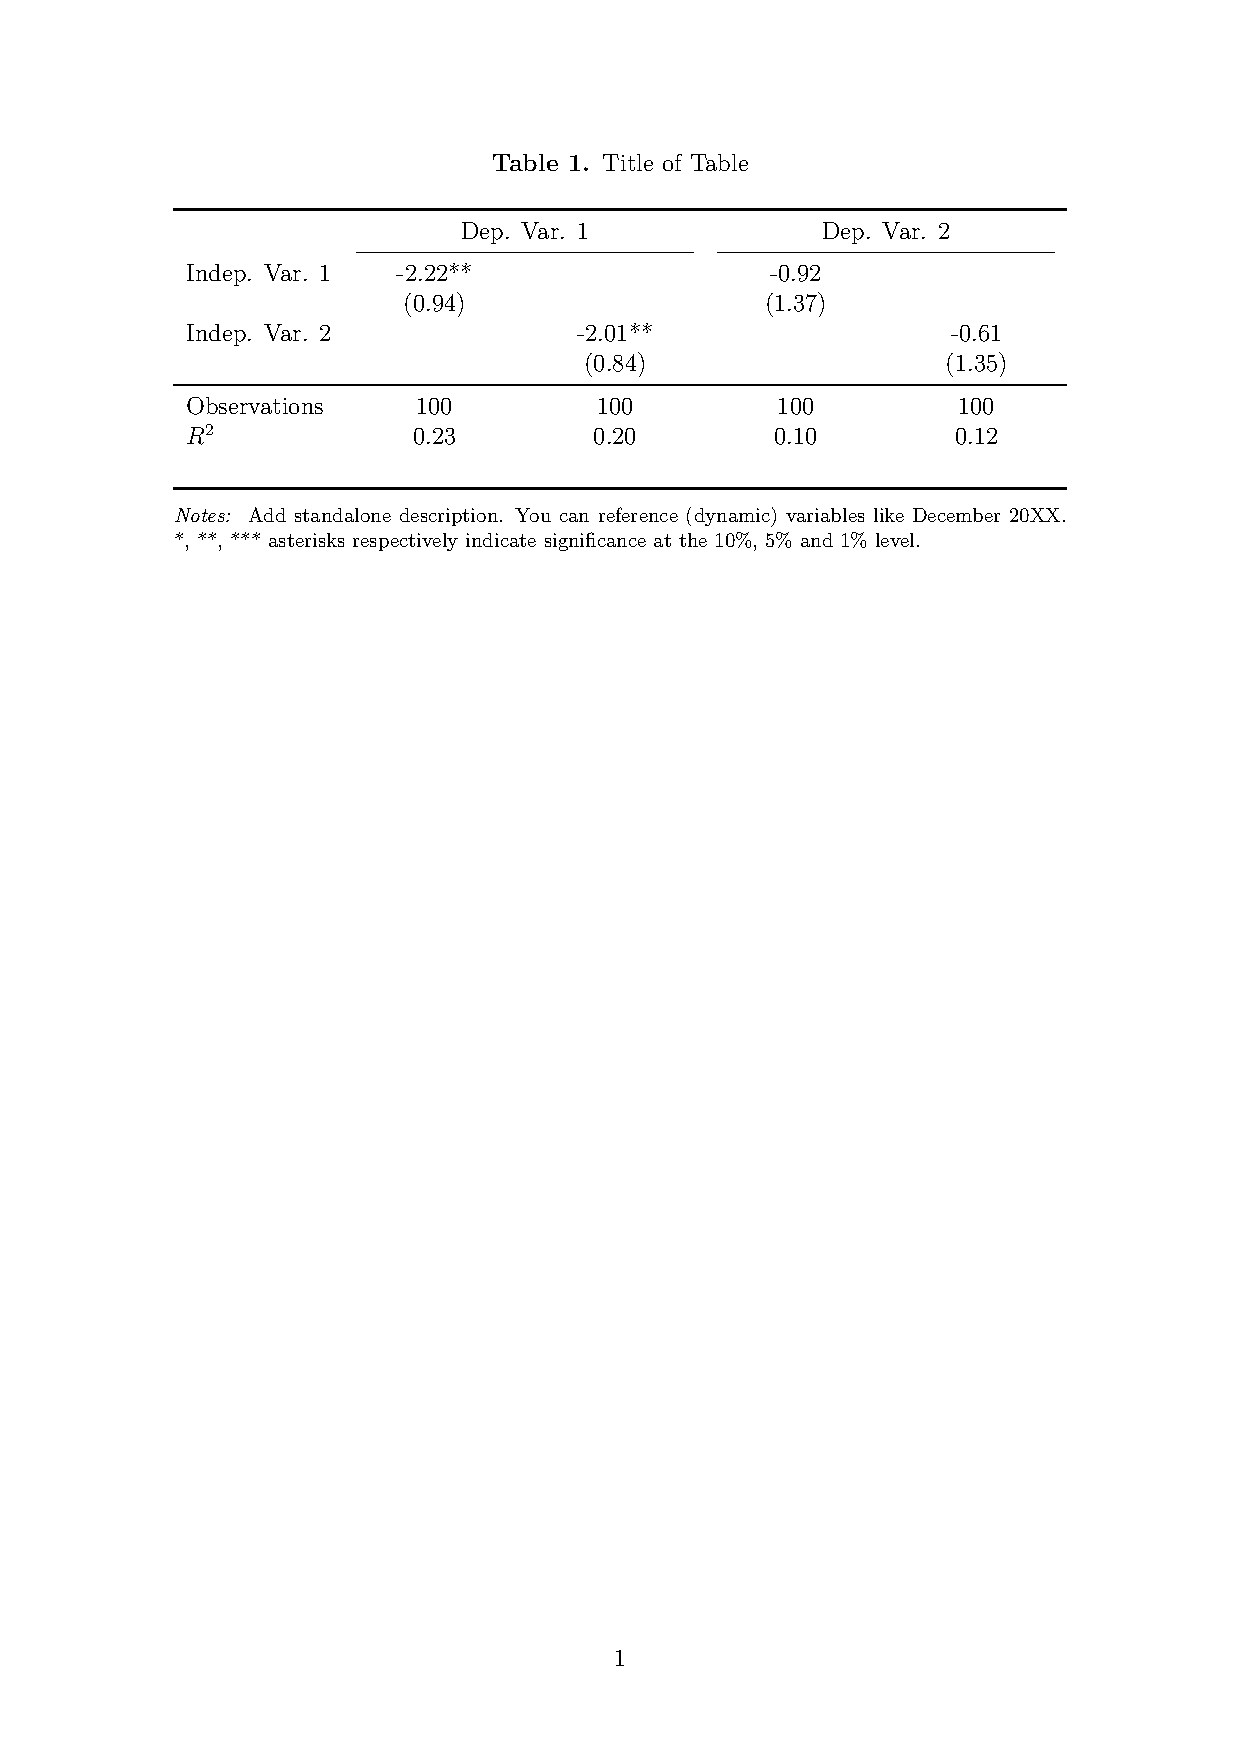
\includegraphics[trim={3cm 21.15cm 3cm 3cm},clip,height=5cm,width=\textwidth,keepaspectratio]{../Tables/extabpdf.pdf}
		% trim={<left> <lower> <right> <upper>}
	\end{center}
\end{frame}
\note[itemize]{
	\item Note.
}


\begin{frame}[label=tableex]
	\frametitle{Table from Paper \uncover<\iftoggle{stops}{2-}{1}>{(Highlighted)}}
	\vspace{-0.25cm}
	\hspace{0.55cm}
	\begin{tikzpicture}
	\node (table) at (0,0)
		{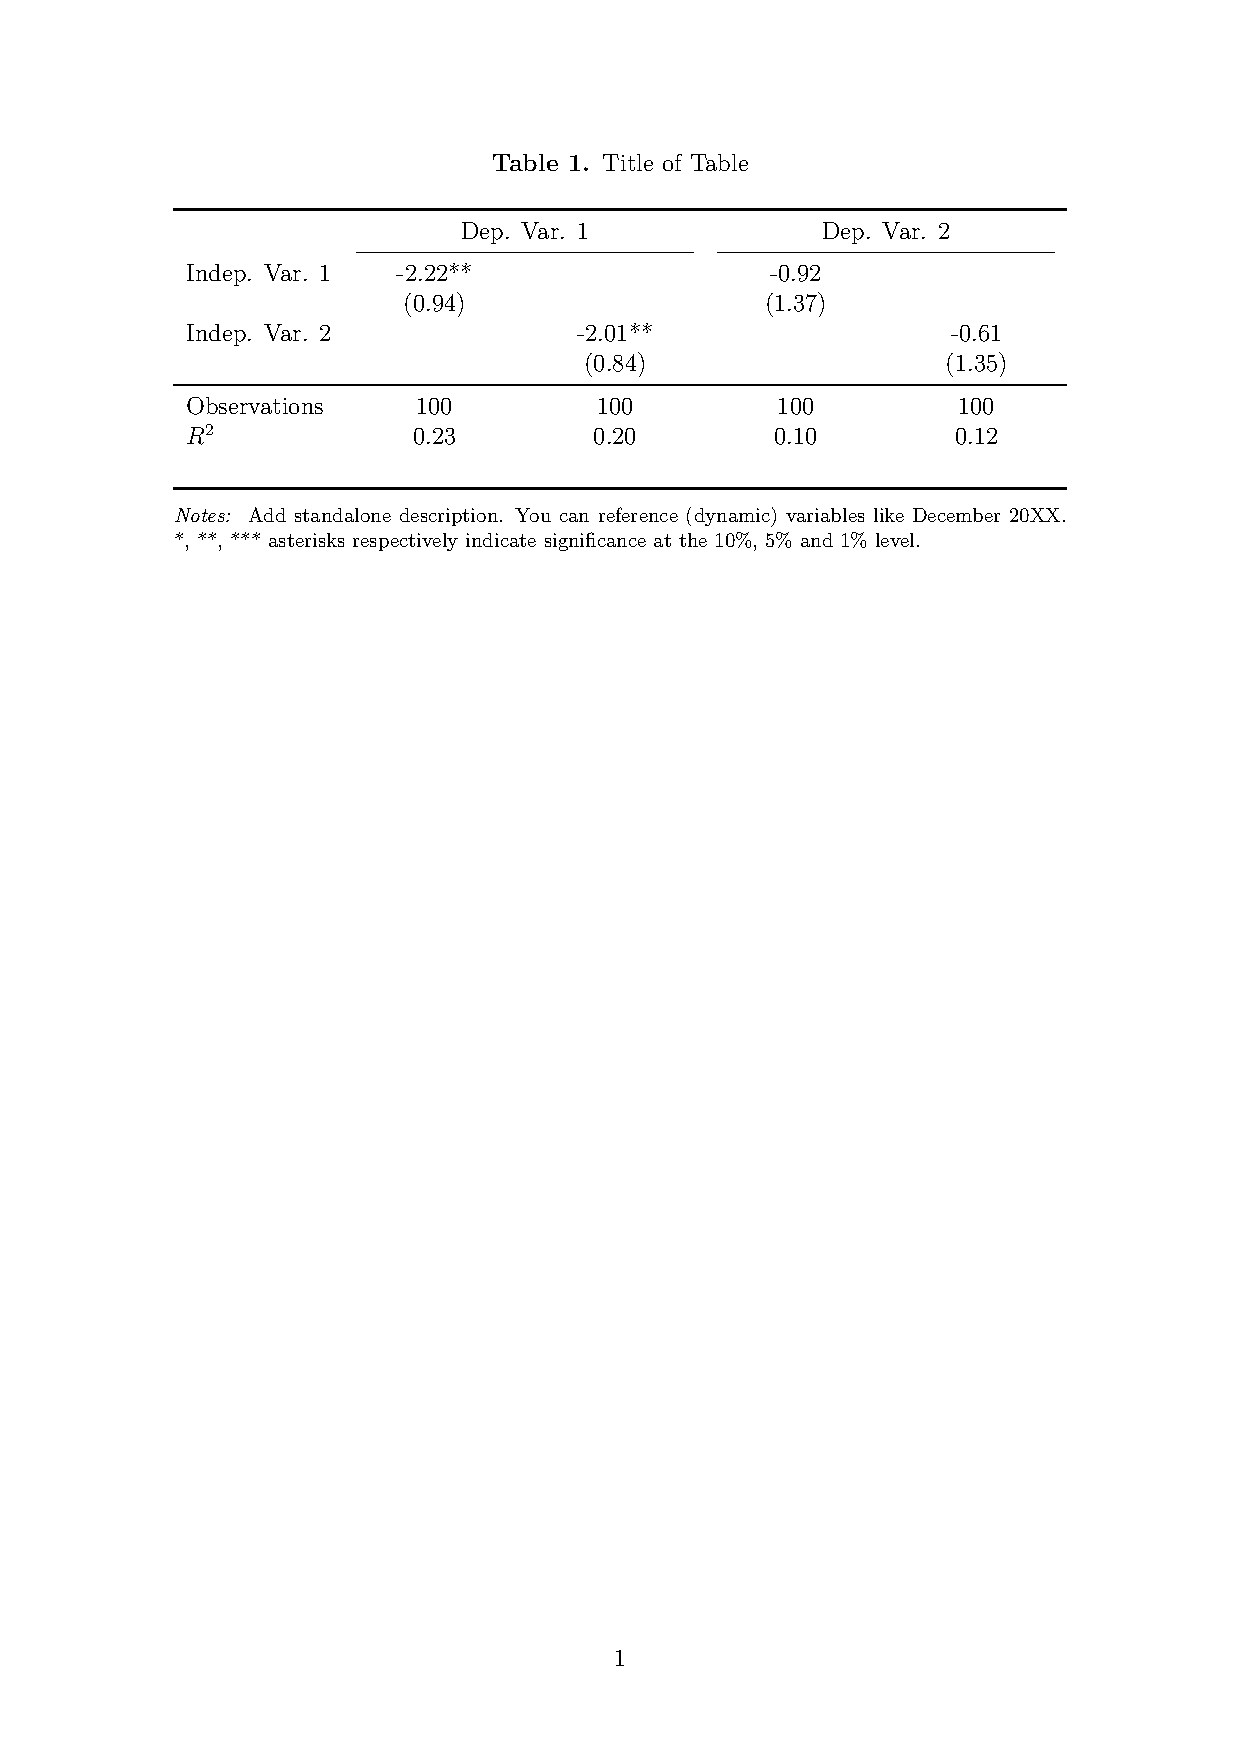
\includegraphics[trim={3cm 21.15cm 3cm 3cm},clip,height=5cm,width=\textwidth,keepaspectratio]{../Tables/extabpdf.pdf}};
		\uncover<\iftoggle{stops}{2-}{1}>{\draw[red,thick] (-1.2,-0.6) rectangle (0.9,0.6);}
		%\draw[step=1cm,gray,very thin] (-4,-4) grid (6,6);
	\end{tikzpicture}
	
	\begin{textblock*}{3cm}(0.94\textwidth,0.98\textheight)	% Left-right, up-down
		\hyperlink<\iftoggle{stops}{2-}{1}>{examples}{\beamerreturnbutton{Examples}}
	\end{textblock*}
\end{frame}
\note[itemize]{
	\item Note.
}


%----------------------------------------------------------------
% Section
%----------------------------------------------------------------
\section*{Appendix}
\appendix

{ \setbeamercolor{page number in head/foot}{fg=date in head/foot.bg} % Hide frame number
\begin{frame}[noframenumbering]
	\begin{center}
		\huge \textcolor{yaleblue}{Appendix}
	\end{center}
\end{frame} }

\begin{frame}[label=figureex]
	\frametitle{Figure from Paper: I}
	\begin{center}
		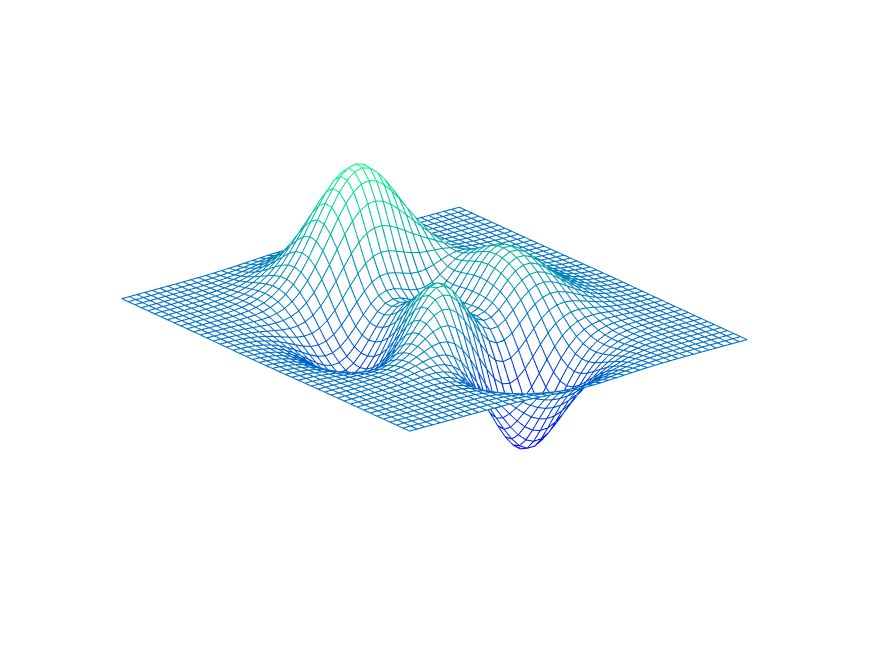
\includegraphics[trim={0cm 0cm 0cm 1cm},clip,height=0.85\textheight,width=\textwidth,keepaspectratio]{../Figures/exfigure1}
		% trim={<left> <lower> <right> <upper>}
	\end{center}
	
	\begin{textblock*}{3cm}(0.94\textwidth,0.6\textheight)	% Left-right, up-down
		\hyperlink{examples}{\beamerreturnbutton{Examples}}
	\end{textblock*}
\end{frame}
\note[itemize]{
	\item Note.
}

\begin{frame}
	\frametitle{Figure from Paper: II}
	\begin{columns}[T] 										% Align columns
		\begin{column}{0.38\textwidth}
			\begin{itemize}
				\item[]
				\item Remark 1
				\item Remark 2
				\item Remark 3
			\end{itemize}
		\end{column}
	\hfill
		\begin{column}{0.58\textwidth}
			\begin{center}
				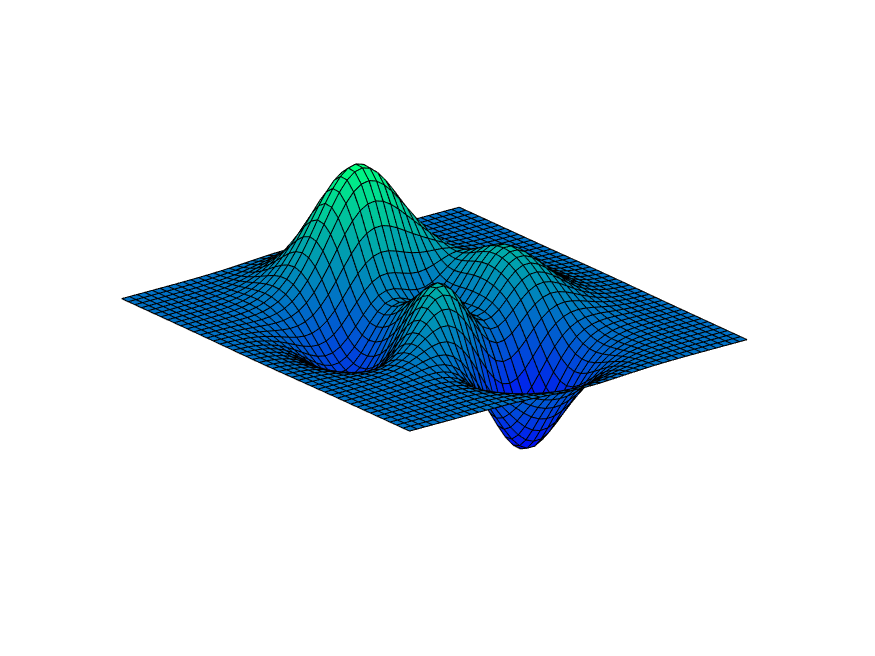
\includegraphics[trim={0cm 0cm 0cm 2.7cm},clip,height=\textheight,width=1.2\textwidth,keepaspectratio]{../Figures/exfigure2}
				% trim={<left> <lower> <right> <upper>}
			\end{center}
		\end{column}%
	\end{columns}

	\begin{textblock*}{3cm}(0.8\textwidth,0.95\textheight)	% Left-right, up-down
		\hyperlink{examples}{\beamerreturnbutton{Examples}}
	\end{textblock*}
\end{frame}
\note[itemize]{
	\item Note.
}


\begin{frame}<0>[noframenumbering]							% Process bib file without adding a slide
%	\printbibliography										% Option 1
	\bibliographystyle{abbrvnat}							% Option 2
	\bibliography{../References/library}					% Option 2
\end{frame}

\end{document}